\documentclass[AMA,Times1COL]{WileyNJDv5} %STIX1COL,STIX2COL,STIXSMALL


\articletype{Original Research}%

\received{Date Month Year}
\revised{Date Month Year}
\accepted{Date Month Year}
\journal{Journal}
\volume{00}
\copyyear{2025}
\startpage{1}

\raggedbottom



\begin{document}

\title{SFM-Unet: A Spatial-Frequency Memorizable Model for Posterior Sclera OCT Analysis}

\author[1]{Jiashu Xu}

\author[2]{Fanglin Chen}

\authormark{Xu \textsc{et al.}}
\titlemark{SFM-Unet: A Spatial-Frequency Memorizable Model for Posterior Sclera OCT Analysis}

\address[1]{\orgdiv{School of Science}, \orgname{Harbin Institute of Technology, Shenzhen}, \orgaddress{\state{Guangdong}, \country{China}}}

\address[2]{\orgdiv{School of Computer Science and Technology}, \orgname{Harbin Institute of Technology, Shenzhen}, \orgaddress{\state{Guangdong}, \country{China}}}

\corres{Corresponding author Jiashu Xu and Fanglin Chen. \email{jiashu\_xu@stu.hit.edu.cn}
\email{chenfanglin@hit.edu.cn}}

%\fundingInfo{Text}
%\JELinfo{ejlje}

\abstract[Abstract]{The analysis of posterior scleral images is crucial for understanding the progression of myopia and developing effective interventions. However, due to the subtle edge variations in posterior scleral images and their high memory requirements, existing 3D models face limitations in memory consumption, while 2D models struggle to capture cross-slice spatial information, making it difficult to balance performance and memory usage. Therefore, we propose SFM-Unet, a novel model designed specifically for OCT analysis of the posterior sclera. SFM-Unet integrates frequency and spatial information through a Cross-Slice Spatial-Frequency Memory module, effectively capturing the complex spatial relationships in 3D images. We conducted experiments on a private dataset EyePS2024 and the publicly available BraTS2020 dataset, where SFM-Unet demonstrated competitive performance across all datasets, demonstrating its effectiveness and practicality in posterior sclera OCT analysis.} 

\keywords{OCT, Medical image analysis, Frequency, Sclera} %image typo

\maketitle

\section{Introduction}
As indicated by the World Health Organization (WHO), the prevalence of myopia is on the rise on a global scale, with the number of individuals affected by this condition now exceeding two billion. The prevalence of myopia in Chinese children and adolescents is approximately 84\%\cite{dong2020prevalence}. Scleral biomechanical properties and scleral remodeling, which represent the ultimate aspects of myopic axial growth, constitute important mechanisms and features in the development of myopia. They may also serve as potential indicators for clinical prediction of myopia progression risk and prognosis\cite{Cao2023}. The analysis of images of the posterior sclera of the eye is essential for understanding the progression of myopia and for the development of effective interventions. As a crucial structure that maintains the shape of the eye and resists internal and external pressure, the mechanical properties of the posterior sclera directly influence the morphological changes of the eye, particularly during periods of elevated intraocular pressure and myopic progression. The pathological growth of the eye axis is closely associated with the biomechanical properties of the posterior sclera. The biomechanical properties of the posterior sclera and its pattern of change may serve as a valuable indicator for predicting myopia progression\cite{Ding2015}. Consequently, the study of the deformation behavior of the posterior sclera and its mechanical properties is of significant scientific importance for a comprehensive understanding of the pathogenesis of myopia and provides a crucial reference for the effective prevention and clinical treatment of myopia in the future.

In recent years, the advancement of medical imaging technology has led to the emergence of biomechanical analysis based on imaging data as a primary investigative tool in the study of the mechanical properties of the eye\cite{li2022simultaneous, koprowski2017new}. In particular, optical coherence tomography (OCT) technology, which is capable of providing high-resolution three-dimensional image data of the posterior part of the eye, has become an important tool for analyzing the mechanical behavior of the sclera.Currently, most of the studies utilising OCT data focus on 2D deep learning architectures\cite{kugelman2019automatic, read2019choroidal}. However, the deformation data of the sclera in the posterior part of the eye is typically presented in three-dimensional or volumetric formats.When 3D images are sliced and processed using models with 2D architectures, the models often fail to effectively capture spatial information across the slices, which may lead to errors when processing complex structures or low-contrast regions.

In order to more effectively analyze 3D medical image data, ÇİÇEK et al.\cite{cciccek20163d} proposed a variant of Unet for processing 3D data, in which 3D convolution is employed to process the spatial information of 3-dimensional data. Similarly, Dou et al.\cite{dou20163d} proposed the 3D Deep Supervision Network (3D DSN) for volume learning and inference. While these methods have yielded promising outcomes, the direct processing of three-dimensional data places a considerable burden on memory, potentially impeding its optimal functioning on certain lower-configuration machines.

Moreover, the majority of extant models operate primarily within the spatial domain, thereby potentially overlooking the crucial information embedded within the frequency domain. Information in the frequency domain can reveal periodic patterns and global features in an image, which helps to capture information that is difficult to distinguish in the spatial domain\cite{huang2023fvfsnet,hai2022combining}, such as texture, edge, and periodic structural features, which are very valuable for accurately capturing subtle changes. In the posterior sclera, deformations are often the result of the accumulation of small, subtle changes over time. The spatial features in a single OCT image may only exhibit minimal variations, making them challenging to capture accurately. However, in the frequency domain, these subtle features tend to cluster around similar frequencies, making them easier to detect and analyze.

In addition, the sclera is composed of dense collagen fibres and elastic fibres\cite{campbell2021biomechanical}. When the stress exceeds the normal physiological range, alterations in the histology of the sclera occur, accompanied by changes in the number and diameter of the collagen fibers, which in turn give rise to modifications in the biomechanical properties of the sclera\cite{yasir2024scleral}. 

To more effectively extract texture and subtle edge changes in ocular images and obtain more precise mechanical properties, we propose new variant of Unet, SFM (Spatial-Frequency Storage) Unet, which combines frequency features and an Enhanced Cross-Slice Spatial-Frequency Memory Block (ECSFMB) module to better extract texture details from ocular images. Our method uses Fourier transform to extract frequency features from the input image and fuses them with spatial features extracted by Unet encoder, which can utilize local and global contextual information to enhance the segmentation ability of complex structured targets. 

Furthermore, we introduce the ECSFMB module at the bottleneck layer of Unet to address cross-slice dependencies between multiple slices in three-dimensional images. By capturing bidirectional dependencies between slices, ECSFMB enhances the consistency and accuracy of segmentation, particularly in regions where cross-slice continuity is paramount. The incorporation of this module enables the model to more effectively capture spatial-frequency features in 3D medical images while maintaining computational efficiency.

In summary, our contributions are as follows:
\begin{itemize}
    \item We propose an enhanced Cross Slice Spatial Frequency Storage Block (ECSFMB) Module, which can better capture the continuity between multiple slices in 3D images, improves the consistency and accuracy of segmentation.
    \item We propose a new variant of Unet, SFM (Spatial Frequency Memory) Unet, which fully utilizes the periodicity and globality of frequency domain features, and integrates frequency features into the ECSFMB module through the Frequency Feature Fusion (FFF) method, paying more attention to the detailed features of complex eye images.
    \item We conducted extensive performance evaluations of the proposed model. The results demonstrate that our model achieves an optimal balance between performance and computational efficiency, validating its effectiveness and practicality.
\end{itemize}


\section{Related work}
\subsection{OCT in prediction of Myopia}
In recent years, optical coherence tomography (OCT) has emerged as a cornerstone technology in myopia research due to its high-resolution and non-invasive imaging capabilities. By utilizing near-infrared light to generate cross-sectional images of posterior sclera, retina, and choroid, this technique provides crucial insights into myopia progression mechanisms\cite{zuo2025machine}. Liu et al. \cite{liu2023posterior} pioneered the application of triple-input polarization-sensitive OCT (TRIPS-OCT) for quantitative assessment of posterior scleral birefringence (PSB), establishing this parameter as a novel biomarker for myopia development. Investigating pediatric high myopia, Tanaka et al.\cite{tanaka2019posterior} conducted ultra-widefield OCT examinations on 55 eyes from 30 patients, revealing posterior staphyloma formation in 12.7\% of cases with characteristic progressive choroidal thinning-thickening alternations at staphyloma margins. Ng et al. \cite{ng2016advances} systematically reviewed OCT applications in pathological myopia, demonstrating its precision in detecting structural alterations spanning from vitreous body to posterior sclera.
\subsection{AI-Driven Prediction with OCT}
The integration of artificial intelligence has significantly advanced OCT image analysis\cite{zuo2025machine}. Li et al. \cite{li2024accurate} developed a multiple linear regression model that achieved accurate prediction of pediatric myopia progression and high myopia risk, demonstrating robust accuracy and generalizability in both internal and external validations. Oh et al. \cite{oh2024prediction} innovatively employed convolutional neural networks (CNN) to establish an axial length prediction system based on macular OCT scans, achieving exceptional performance across validation cohorts and offering new perspectives on retina-choroid complex interactions with axial elongation. These advancements collectively highlight the transformative potential of OCT data combined with machine learning in myopia management.

\section{Methodology}
\subsection{Model Overview}
The overview of SFM-Unet is shown in Fig.~\ref{fig:1}. We utilize Fourier transform to extract frequency-domain features from the input image, and fuse the frequency-domain features with the spatial features extracted by the encoder through FFF (frequency feature fusion) method to obtain comprehensive local and global features. Then, through ECSFMB (Enhanced Cross-Slice Spatial-Frequency Memory Block), we focus on the cross slice dependencies between multiple slices in 3D images, further enhancing the spatiotemporal features in 3D medical images.

\begin{figure*}[htbp]
\centerline{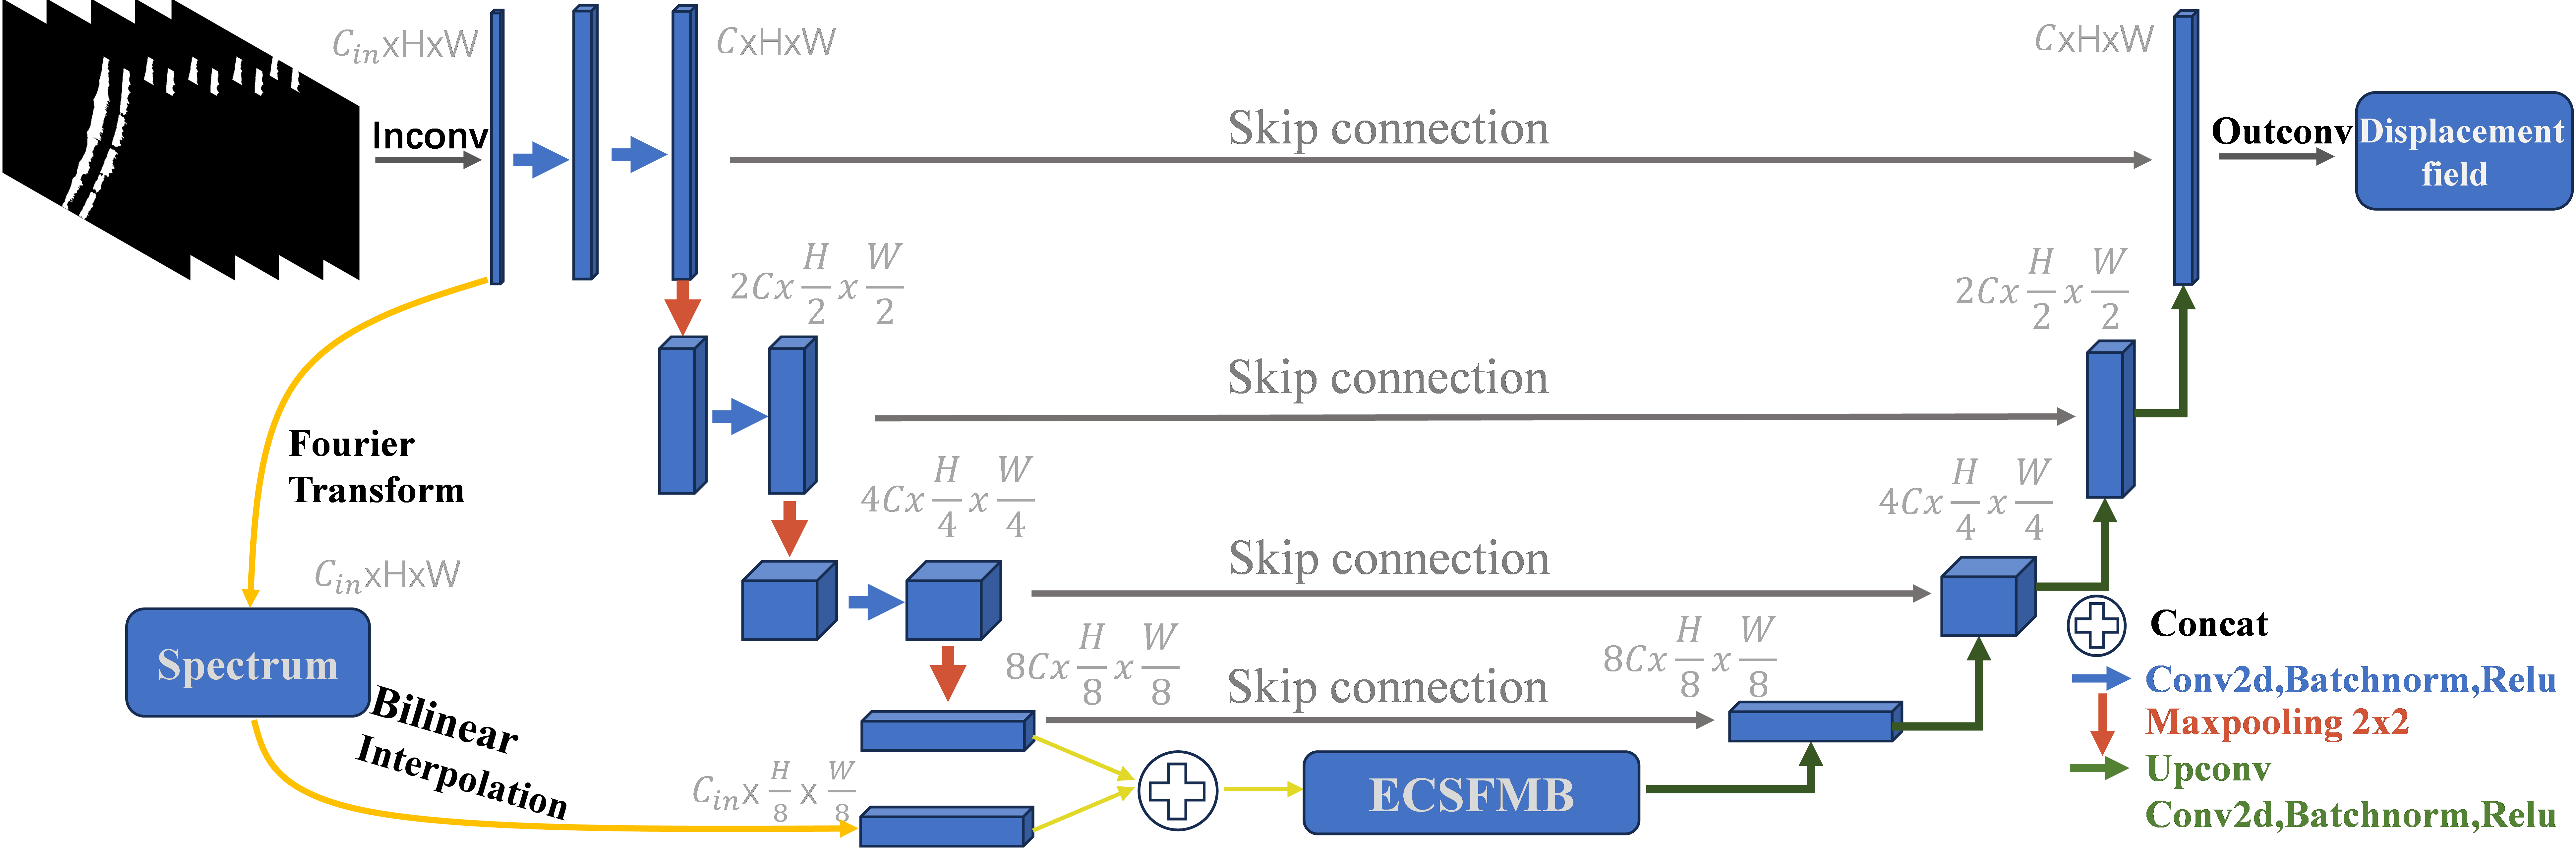
\includegraphics[width=0.95\linewidth]{Fig/fig1.png}}
\caption{Model structure of SFM-Unet}
\label{fig:1}
\end{figure*}

\subsection{Frequency feature fusion(FFF)}
In the posterior sclera OCT image and the posterior sclera mechanically loaded OCT image, the mechanically changing characteristics of myopia manifest as minor alterations in the image. These alterations typically necessitate the integration of global information to enhance the precision and accuracy of the assessment. The frequency information of the image is well suited for this purpose. Therefore, we propose a frequency feature fusion (FFF) approach that integrates frequency and spatial domain features to extract a more comprehensive set of local and global information.

Specifically, the feature map \( F(x) \) output from the initial convolutional layer is transformed into the frequency domain using the Fourier transform:
\begin{equation}
\mathcal{F}(u, v) = \sum_{x=0}^{M-1} \sum_{y=0}^{N-1} F(x, y) \cdot e^{-j2\pi\left(\frac{ux}{M} + \frac{vy}{N}\right)},
\end{equation}
where \( M \) and \( N \) are the spatial dimensions of the feature map, and \((u, v)\) are the frequency coordinates.

To focus on global information, we extract the magnitude spectrum:
\begin{equation}
|\mathcal{F}(u, v)| = \sqrt{\text{Re}(\mathcal{F}(u, v))^2 + \text{Im}(\mathcal{F}(u, v))^2},
\end{equation}
where \( \text{Re}(\cdot) \) and \( \text{Im}(\cdot) \) represent the real and imaginary parts of the frequency components, respectively.

The frequency features obtained by Fourier transform are spliced with the spatial features extracted by the encoder at a later stage in the channel dimension, thereby enhancing the accuracy of the segmentation process for complex structures and low-contrast regions.

\subsection{Enhanced Cross-Slice Spatial-Frequency Memory Block (ECSFMB)}
The Enhanced Cross-Slice Spatial-Frequency Memory Block (ECSFMB) is designed to effectively capture cross-slice dependencies and spatial-frequency information in 3D medical images. Unlike conventional methods that process slices independently, the ECSFMB models bidirectional dependencies across slices while maintaining critical spatial and frequency features.The structure of the ECSFMB module is illustrated in Fig~\ref{fig:2}.

\begin{figure}[htbp]
\centerline{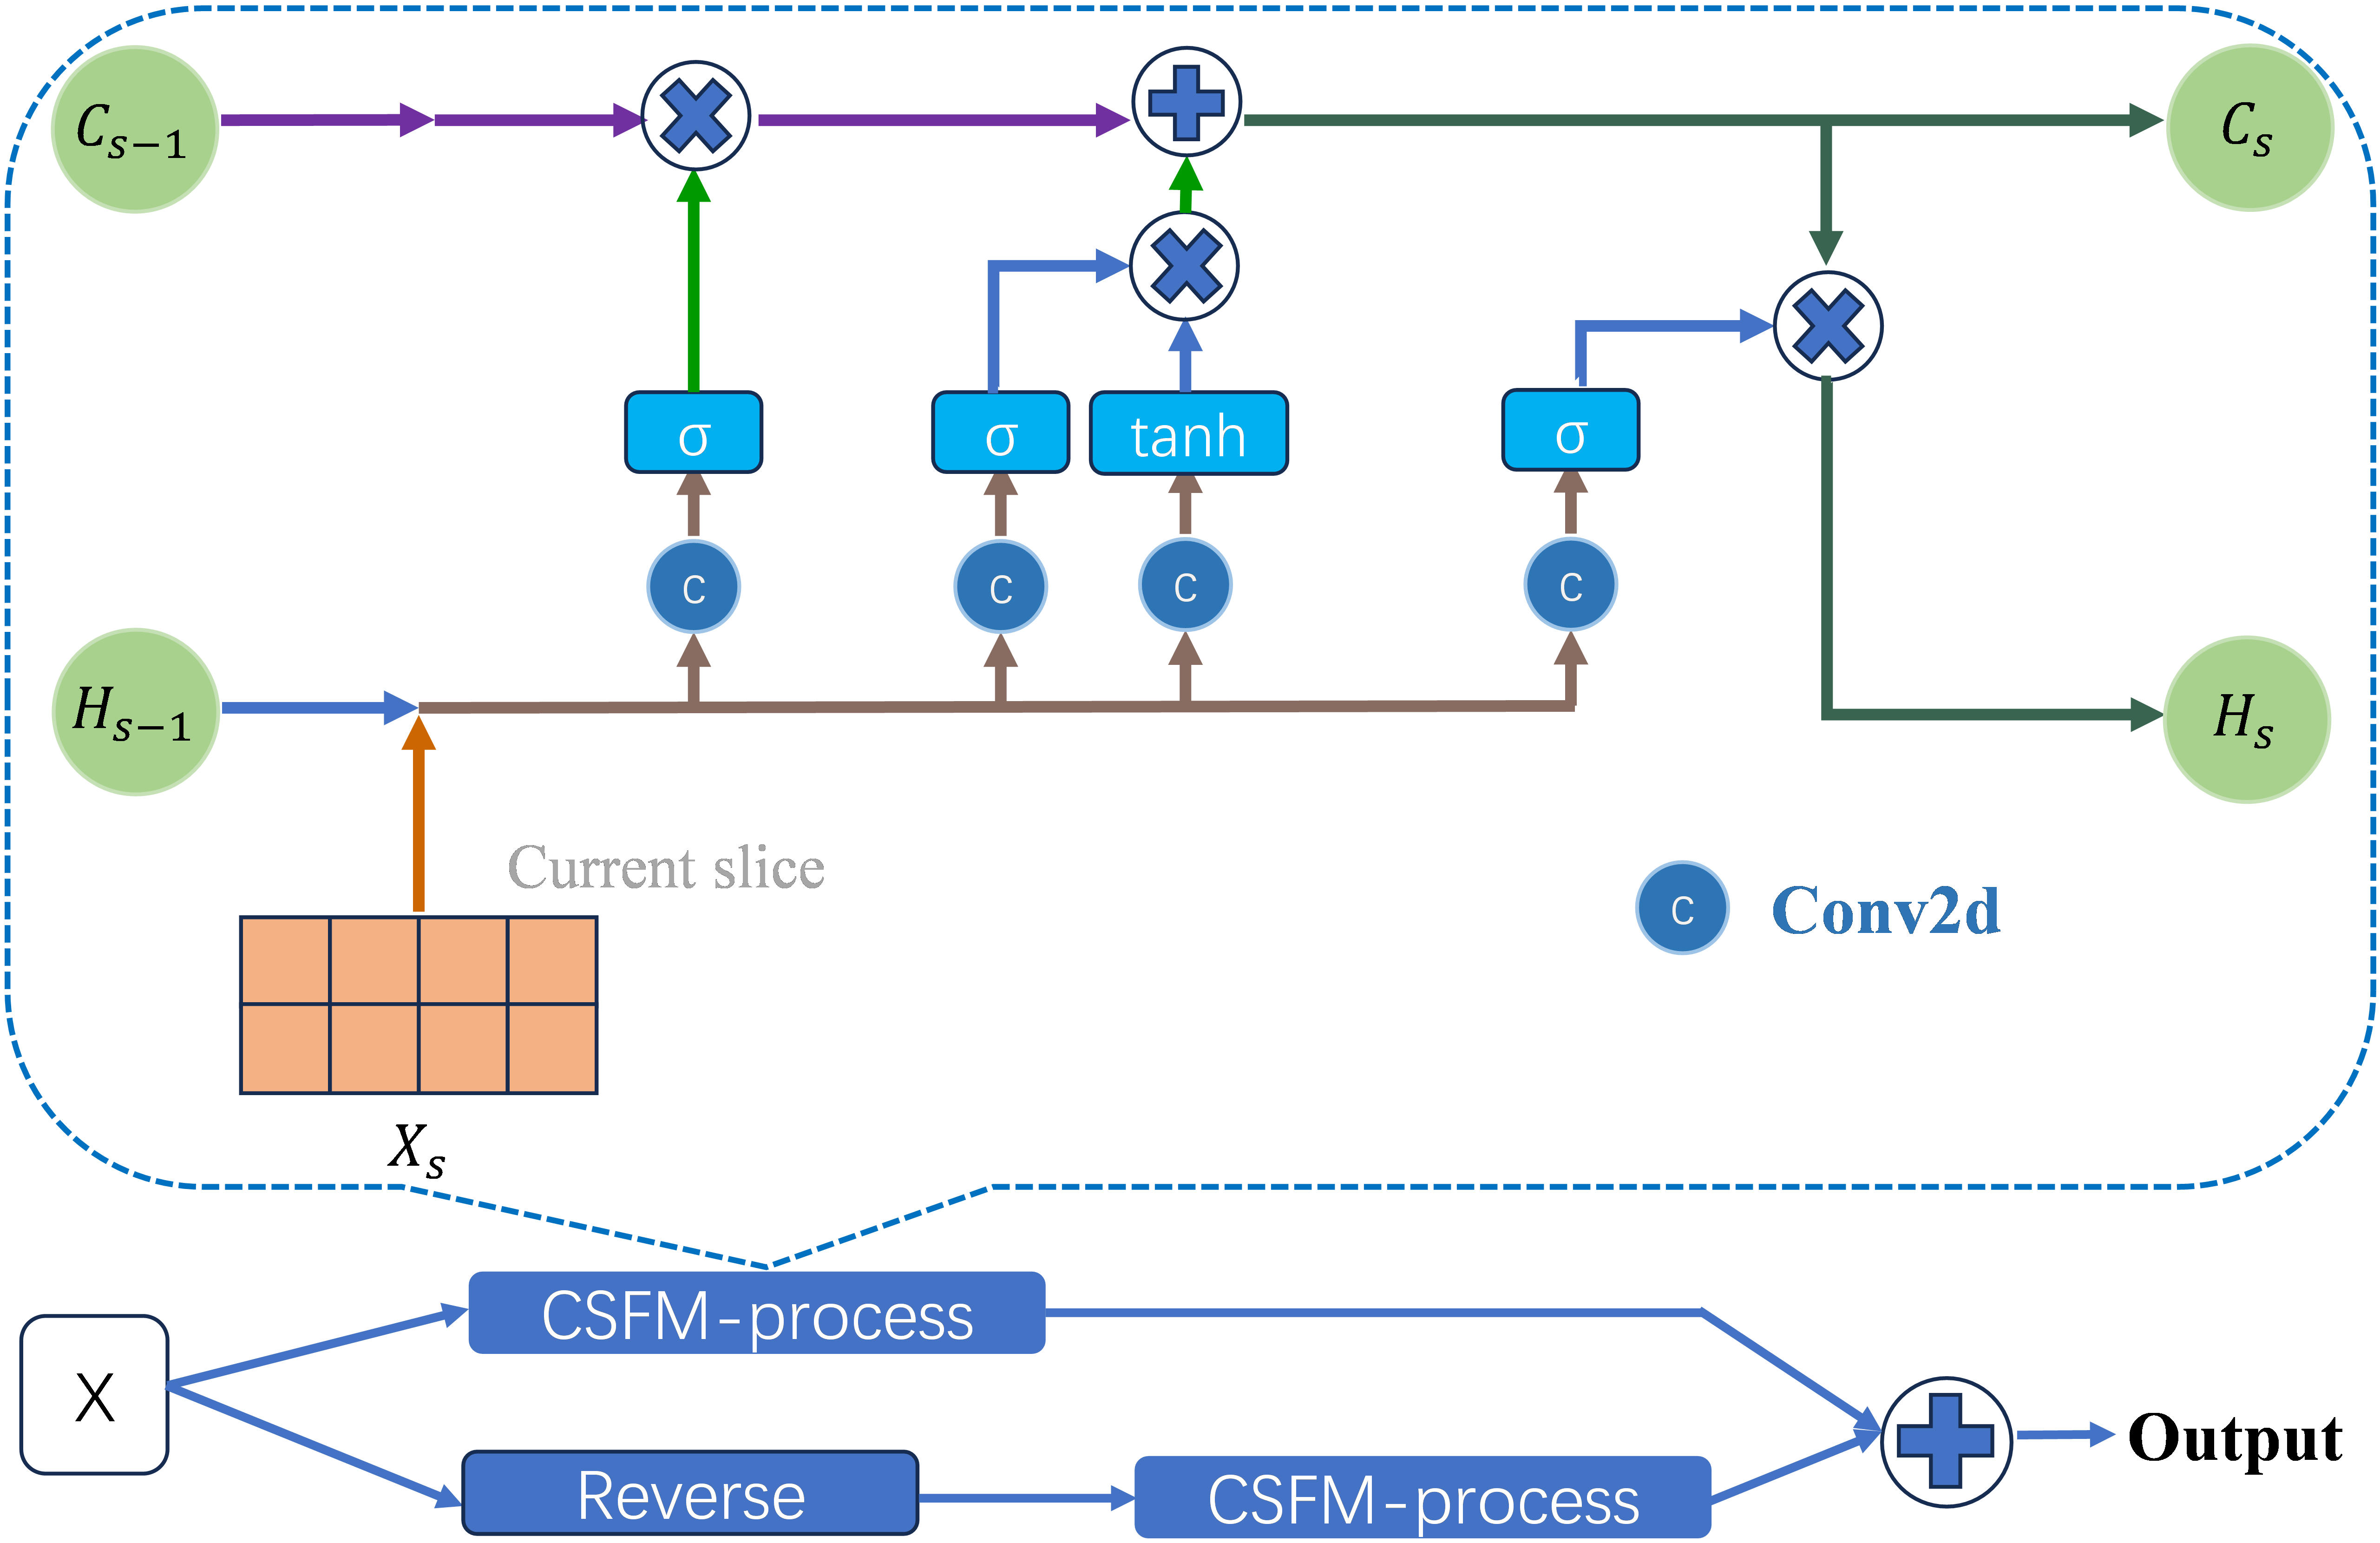
\includegraphics[width=0.75\linewidth]{Fig/fig2.png}}
\caption{Schematic structure of ECSFMB}
\label{fig:2}
\end{figure}

Specifically, ECSFMB processes input slices $X_s$ through convolutional operations, thereby generating enhanced feature representations based on two-way dependency modelling. For each slice \( X_s \), the feature representations are computed using a gated mechanism to capture spatial and contextual information. The computation process unfolds as follows:

First, the contribution of the previous state \( C_{s-1} \) to the current state is determined using a gating mechanism:
\begin{equation}
    f_s = \sigma(W_f \ast X_s + U_f \ast C_{s-1} + b_f),
\end{equation}

Next, the extent to which new information from the current slice \( X_s \) should be added to the state is computed:
\begin{equation}
    i_s = \sigma(W_i \ast X_s + U_i \ast C_{s-1} + b_i),
\end{equation}

Subsequently, the potential update for the current state is calculated based on the input features:
\begin{equation}
    g_s = \tanh(W_g \ast X_s + U_g \ast C_{s-1} + b_g),
\end{equation}

Finally, the feature representation \( C_s \) for the current slice is updated as:
\begin{equation}
    C_s = f_s \odot C_{s-1} + i_s \odot g_s,
\end{equation}
where \( \odot \) denotes element-wise multiplication, ensuring the fusion of retained past information and new features.

The forward representation \( C_s \) for the current slice is then propagated to subsequent layers. A similar process can be applied in the reverse direction to model backward dependencies. For bidirectional processing, the final cross-slice representation \( C_s \) is obtained by combining forward and backward features: 
\begin{equation}
   C_s = \overrightarrow{C_s} + \overleftarrow{C_s} 
\end{equation}

Subsequently, the features are recovered as high-resolution segmentation maps by a decoder, while maintaining crucial spatial data and temporal consistency. 

\subsection{Loss function}
We employ the Diceloss and Cross-entropy loss function, which are the most elementary in medical image analysis. We then combine these two elements. By calculating the loss at the batch level, we have devised a loss function that can mitigate the fluctuations in loss observed for individual samples, which may be attributable to random noise or misclassification of minor structures. This enables the model to converge in a more stable manner. Furthermore, it can enhance the overall segmentation performance, particularly in scenarios where data distribution is uneven, and facilitate more accurate weighting of different samples. The specific loss function is presented in \eqref{equ:loss}. $\alpha$ refer to the weights of loss functions, which is set to $0.5$ by default.

\begin{equation}
\label{equ:loss}
\left\{
\begin{aligned}
\text{Loss}_{\text{batch}} &= (1-\alpha)\times\text{CE}_{\text{batch}}+\alpha\times\text{DiceLoss}_{\text{batch}} \\
\mathrm{CE}_{\mathrm{batch}} &= -\frac{1}{B}\sum_{b=1}^{B}\text{Target}_{b}\log(\text{Input}_{b}) \\
\mathrm{Diceloss}_{\mathrm{batch}} &= 1-\frac{2\sum_{b=1}^{B}\mathrm{Input}_{b}^{}\times\mathrm{Target}_{b}^{}}{\sum_{b=1}^{B}\left(\mathrm{Input}_{b}^{}+\mathrm{Target}_{b}^{}\right)+\epsilon}
\end{aligned}
\right.
\end{equation}

\section{Experiment}
\subsection{Datasets}
\textbf{EyePS2024}: We utilized the EyePS2024 dataset, a private dataset of posterior sclera mechanics under mechanical loading. The dataset comprises 192 labeled cases, each of which consists of a baseline image and a mechanical loading image. Both the baseline and mechanical loading images are 3D OCT scans in DICOM format. Each case contains a displacement field as a label, which characterizes the posterior scleral biomechanical compliance as either high or low, which can be an important predictor of myopia progression.

\textbf{Brats2020}: We utilized BraTS2020 dataset\cite{menze2014multimodal-brats1}\cite{bakas2017advancing-brats2}, which is a publicly available, large-scale brain multimodal MRI glioma segmentation dataset. The dataset includes 369 labeled training cases and 125 unlabeled validation cases. Each training case comprises 3D images of four modalities and one unified label. The annotations include GD-enhancing tumor, peritumoral edematous, and necrotic tumor core.

\subsection{Evaluation Metrics}
For the EyePS2024 dataset, following established protocol in ophthalmic image analysis\cite{oh2024prediction}, we employ Mean Squared Error (MSE) and Mean Absolute Error (MAE) as primary evaluation metrics, which are written as:

\begin{equation}
\begin{aligned}
    \text{MSE} &= \frac{1}{N}\sum_{i=1}^{N}(y_i - \hat{y}_i)^2 \\
    \text{MAE} &= \frac{1}{N}\sum_{i=1}^{N}|y_i - \hat{y}_i|
\end{aligned}
\end{equation}

where $y_i$ denotes the ground-truth value, $\hat{y}_i$ represents the predicted value, and N is the total number of pixels/voxels. MSE quantifies the overall magnitude of prediction errors with quadratic weighting, particularly sensitive to large deviations, while MAE provides a robust linear measure of absolute pixel-wise discrepancies, ensuring balanced evaluation across heterogeneous anatomical structures.

For the BraTS2020 dataset, consistent with brain tumor segmentation benchmarks\cite{menze2014multimodal,chen2024adaptive}, we employed the Dice coefficient (Dice) and 95\% Hausdorff Distance (HD95) as major metrics to evaluate the segmentation accuracy, which are written as:
\begin{equation}
    \mathrm{Dice}=\frac{2\times|A\cap B|}{|A|+|B|}
\end{equation}

\begin{equation}
\mathrm{HD95}=\max\left\{\sup_{a\in\partial A}\inf_{b\in\partial B}\|a-b\|,\sup_{b\in\partial B}\inf_{a\in\partial A}\|b-a\|\right\}_{95\%}
\end{equation}

where, A and B denote the predicted and ground-truth segmentation masks, respectively. We use Dice to evaluate the overlap between the predicted segmentation (A) and the ground truth (B) on a pixel-by-pixel basis. Hausdorff Distance (HD95) measures the boundary discrepancy between the predicted segmentation and the ground truth, highlighting the precision of boundary localization.

\subsection{Implementation details}
SFM-Unet is implemented on a NVIDIA RTX 3090 GPU with 24 GB VRAM using the open source PyTorch framework. To complicate the data distribution and mitigate the overfitting problem, we applied various data augmentation methods in the preprocessing stage, including random scaling (0.9-1.1), random flipping in three directions (axial/sagittal/coronal), random rotation ($\pm 15^\circ$), introduction of Gaussian noise ($\sigma = 0.01$), and random contrast (0.8-1.2 ratio). 

To ensure a fair comparison with state-of-the-art (SOTA) methods, we meticulously reimplemented all baseline models on our local machine under identical experimental settings, including hardware configuration, data preprocessing pipelines, and evaluation protocols. 

The initial learning rate was set to 5e-4, and a warm-up strategy was employed to linearly increase the learning rate to 0.01 within the first ten training cycles. Thereafter, the learning rate was tuned using a cosine annealing algorithm in accordance with \eqref{lr-equ}. The number of epochs for model training was set to 300, and the objective function was defined as before.
\begin{equation}
    \label{lr-equ}
    lr = 0.01 \times \left(1 + \cos\left(\frac{\pi \times \text{step}}{\text{decay steps}}\right)\right)
\end{equation}

\subsection{Comparison with SOTA models}
% 添加说明不使用dice等分割指标的原因
We first conducted experiments on the EyePS2024 dataset, in which SFM-Unet was compared with several state-of-the-art models. As shown in Table~\ref{tab:mae_mse_comparison}, SFM-Unet achieves the lowest mean absolute error (MAE) of 0.042 and a mean squared error (MSE) of 3.038,which is on par with the best-performing TransUNet. Meanwhile, SFM-Unet notably surpasses other state-of-the-art models, including Unet, UNet++, and Res-UNet. This demonstrates the superior capability of SFM-Unet to accurately model the deformation field of the sclera in the EyePS2024 dataset.

In terms of parameter efficiency, SFM-Unet demonstrates a significant advantage. With only 5.51M parameters, SFM-Unet is the most compact model among those evaluated, while still maintaining top-tier performance. In comparison, models like TransUNet and Swin-UNet have significantly higher parameter counts, with 105.28M and 27.17M parameters, yet they do not offer a notable improvement in accuracy, thereby highlighting the efficiency of SFM-Unet.

\begin{table}[htbp]
\scriptsize
\centering
\caption{Comparison with state-of-the-art models on EyePS2024.(\textbf{Bold} indicates the best.)}
\begin{tabular}{lcccc}
\toprule
\textbf{Model} & \textbf{Venue} & \textbf{MAE$\downarrow$} & \textbf{MSE$\downarrow$}  & \textbf{Parameters(M)$\downarrow$}\\
\midrule
UNet\cite{ronneberger2015u}  & MICCAI'15   & 0.125  & 6.038 & 3.71 \\
Res-Unet\cite{xiao2018weighted} & ITME'18 & 0.093  & 4.029 & 6.99 \\
Att-Unet\cite{oktay2018attention} & MIDL'18 & 0.051  & 3.179 & 34.88 \\
Unet++\cite{zhou2019unet++} & TMI'20 & 0.063  & 3.779 & 9.16 \\
Swin-Unet\cite{cao2022swin} & ECCV'22 & 0.042  & 3.035 & 27.17 \\
TransUNet\cite{chen2024transunet} & MIA'24 & 0.042  & \textbf{3.026} & 105.28 \\
Ours(SFM-Unet) & - & \textbf{0.042}  & 3.038 & \textbf{5.51} \\
\bottomrule
\end{tabular}
\label{tab:mae_mse_comparison}
\end{table}

%Since our dataset is private and specifically designed for analyzing the deformation field of the sclera at the back of the eye under mechanical loading, and due to the lack of publicly available, large-scale datasets for such analysis, it is challenging to find a comparable benchmark. %Therefore, we chose to validate the effectiveness and generalization capability of SFM-Unet using the BraTS2020 dataset.

Since our dataset is private and specifically designed for analyzing the deformation field of the sclera at the back of the eye under mechanical loading, and due to the lack of publicly available, large-scale datasets for such analysis, it is challenging to find a comparable benchmark. Due to the fact that EyePS2024 dataset is a 3D image dataset, after analyzing existing publicly available 3D datasets, we believe that the BraTS2020 dataset has certain similarities. Firstly, both BraTS2020 and our dataset consist of high-resolution 3D images, making the performance on BraTS2020 a suitable representation of the potential performance of SFM-Unet in similar tasks. Furthermore, BraTS2020 data are analogous to OCT images, which further supports the adaptability and generalization of the model. Additionally, BraTS2020 provides an official validation platform that allows for direct comparisons using a common test set, offering a standardized and reliable evaluation of our model's performance. Therefore, we chose the BraTS2020 dataset to verify the generalization of our SFM-Unet.

\begin{table*}[htbp]
\centering
\scriptsize
\caption{Comparisons with state-of-the-art models on BraTS 2020 validation cases.The results are calculated through the online evaluation platform, CBICA-IPP. The average of Dice are computed and used for ranking our methods.(\textbf{Bold} indicates the best.)}
\begin{tabular}{lcccccccccccccc}
\toprule
\multirow{2}{*}{Dataset} & \multirow{2}{*}{Model}& \multirow{2}{*}{Venue} & \multicolumn{4}{c}{Dice(\%)} & \multicolumn{4}{c}{Hausdorff95($mm$)} \\ 
\cmidrule(lr){4-7} \cmidrule(lr){8-11}
 & & ET$\uparrow$ & WT$\uparrow$ & TC$\uparrow$ & Mean$\uparrow$ & ET$\downarrow$ & WT$\downarrow$ & TC$\downarrow$ & Mean$\downarrow$ \\ 
\midrule
BraTS2020 & nnUnet\cite{isensee2018nnu}&Nature methods'21 & 82.7 & 80.4 & 86.4 & 83.2 & 39.246 & 8.069 & 12.492 & 19.936 \\ 
 & SwinBTS\cite{jiang2022swinbts}&Brain Sciences'22 & 77.6 & 89.2 & 80.4 & 82.4 & 26.840 & 8.560 & 15.780 & 17.060 \\ 
 & TransBTS\cite{wenxuan2021transbts}&MICCAI'21 & 76.6 & 89.0 & 80.4 & 82.0 & 29.830 & 5.600 & \textbf{9.770} & 15.067 \\ 
 & VTU-Net\cite{peiris2022VTU}&MICCAI'22 & 76.7 & 88.9 & 80.5 & 82.0 & 28.990 & 9.560 & 14.400 & 17.650 \\ 
 & SDS-Unet\cite{henry2021brain}&MICCAI &  78.50 & 88.59 & 84.27 & 83.78 & 20.360 & 6.667 & 19.549 & 14.192 \\ 
 & ACTransU-Net\cite{chen2024adaptive}&PMB'24 &  79.58 & \textbf{90.71} &  84.58 &  84.96 & 20.900 & \textbf{5.400} & 11.000 & 12.433 \\ 
 & Ours(SFM-Unet)&- & \textbf{82.8} & 85.9 & \textbf{87.6} & \textbf{85.4} & \textbf{15.872} & 6.133 & 11.401 & \textbf{11.136} \\ 
\bottomrule
\end{tabular}
\label{tab:sota}
\end{table*}

%There are several reasons for selecting BraTS2020. Firstly, both BraTS2020 and our dataset consist of high-resolution 3D images, making the performance on BraTS2020 a suitable representation of the potential performance of SFM-Unet in similar tasks. Furthermore, BraTS2020 data are analogous to OCT images, which further supports the adaptability and generalization of the model. Additionally, BraTS2020 provides an official validation platform that allows for direct comparisons using a common test set, offering a standardized and reliable evaluation of our model's performance. Considering these factors, the experimental results on the BraTS2020 dataset effectively demonstrate the advantages and applicability of SFM-Unet.

Table~\ref{tab:sota} show detailed comparison results for Dice and Hausdorff95 evaluations of our method and the state of-the-art methods, including nnUnet and AttentionUnet, which are commonly utilized for medical image analysis, and networks specifically designed for brain tumor image segmentation, such as TranBTS, SwinBTS, and VTU-net. As illustrated in the table, our proposed model exhibits the optimal performance in terms of dice average and HD95 average on BraTS2020 datasets.

%In the BraTS2020 dataset, only TransBTS outperforms our model in terms of HD95 in the TC region. This advantage can be attributed to the model's innovative approach of extracting local contextual information from 3D space using 3DCNN. While only SwinBTS outperforms our model in terms of DSC on the WT region, this is attributed to the inclusion of the ETrans module, which combines a convolutional neural network (CNN) and the Transformer structure at the bottom of the model. However, our model still performs the best in terms of overall performance, indicating that our model has excellent performance in feature learning.
In the BraTS2020 dataset, only TransBTS demonstrates superior performance in HD95 of the tumor core (TC) region compared to our model, which can be attributed to its innovative integration of 3D CNN architecture for extracting local contextual information from three-dimensional spatial features. Regarding the Dice Similarity Coefficient (DSC) in the whole tumor (WT) region, ACTransU-Net marginally outperforms our approach through its implementation of the omni-dimensional dynamic convolution (ODConv) module that adaptively adjusts convolution kernel parameters based on input characteristics, thereby enhancing local tumor boundary delineation. Nevertheless, our model achieves state-of-the-art performance across comprehensive evaluation metrics, demonstrating its exceptional capability in hierarchical feature learning and global context integration. The comparative analysis suggests that while specialized architectures may excel in specific sub-region segmentation tasks through targeted module design, our framework maintains superior generalizability through optimized multi-scale feature representation and cross-modality information fusion.

\subsection{Visualization Results}
To demonstrate the enhanced performance of the SFM-Unet in the analysis of the sclera in the posterior part of the eye, we have visualized and compared one slice from the same case. The results are presented in Fig~\ref{fig:3}. It is evident that UNet exhibits significant errors in certain regions, which are highlighted in red in the figure. Furthermore, a comparison with Res-UNet reveals that in the region delineated by the yellow circle, the output of SFM-Unet is more closely aligned with the actual labeling (ground truth). This visual comparison provides compelling evidence of the efficacy of SFM-Unet in the mechanical analysis of the sclera at the posterior aspect of the eye. This visual representation allows for a more nuanced understanding of the advantages of SFM-Unet in processing complex biomedical images.
\begin{figure}[htbp]
\centerline{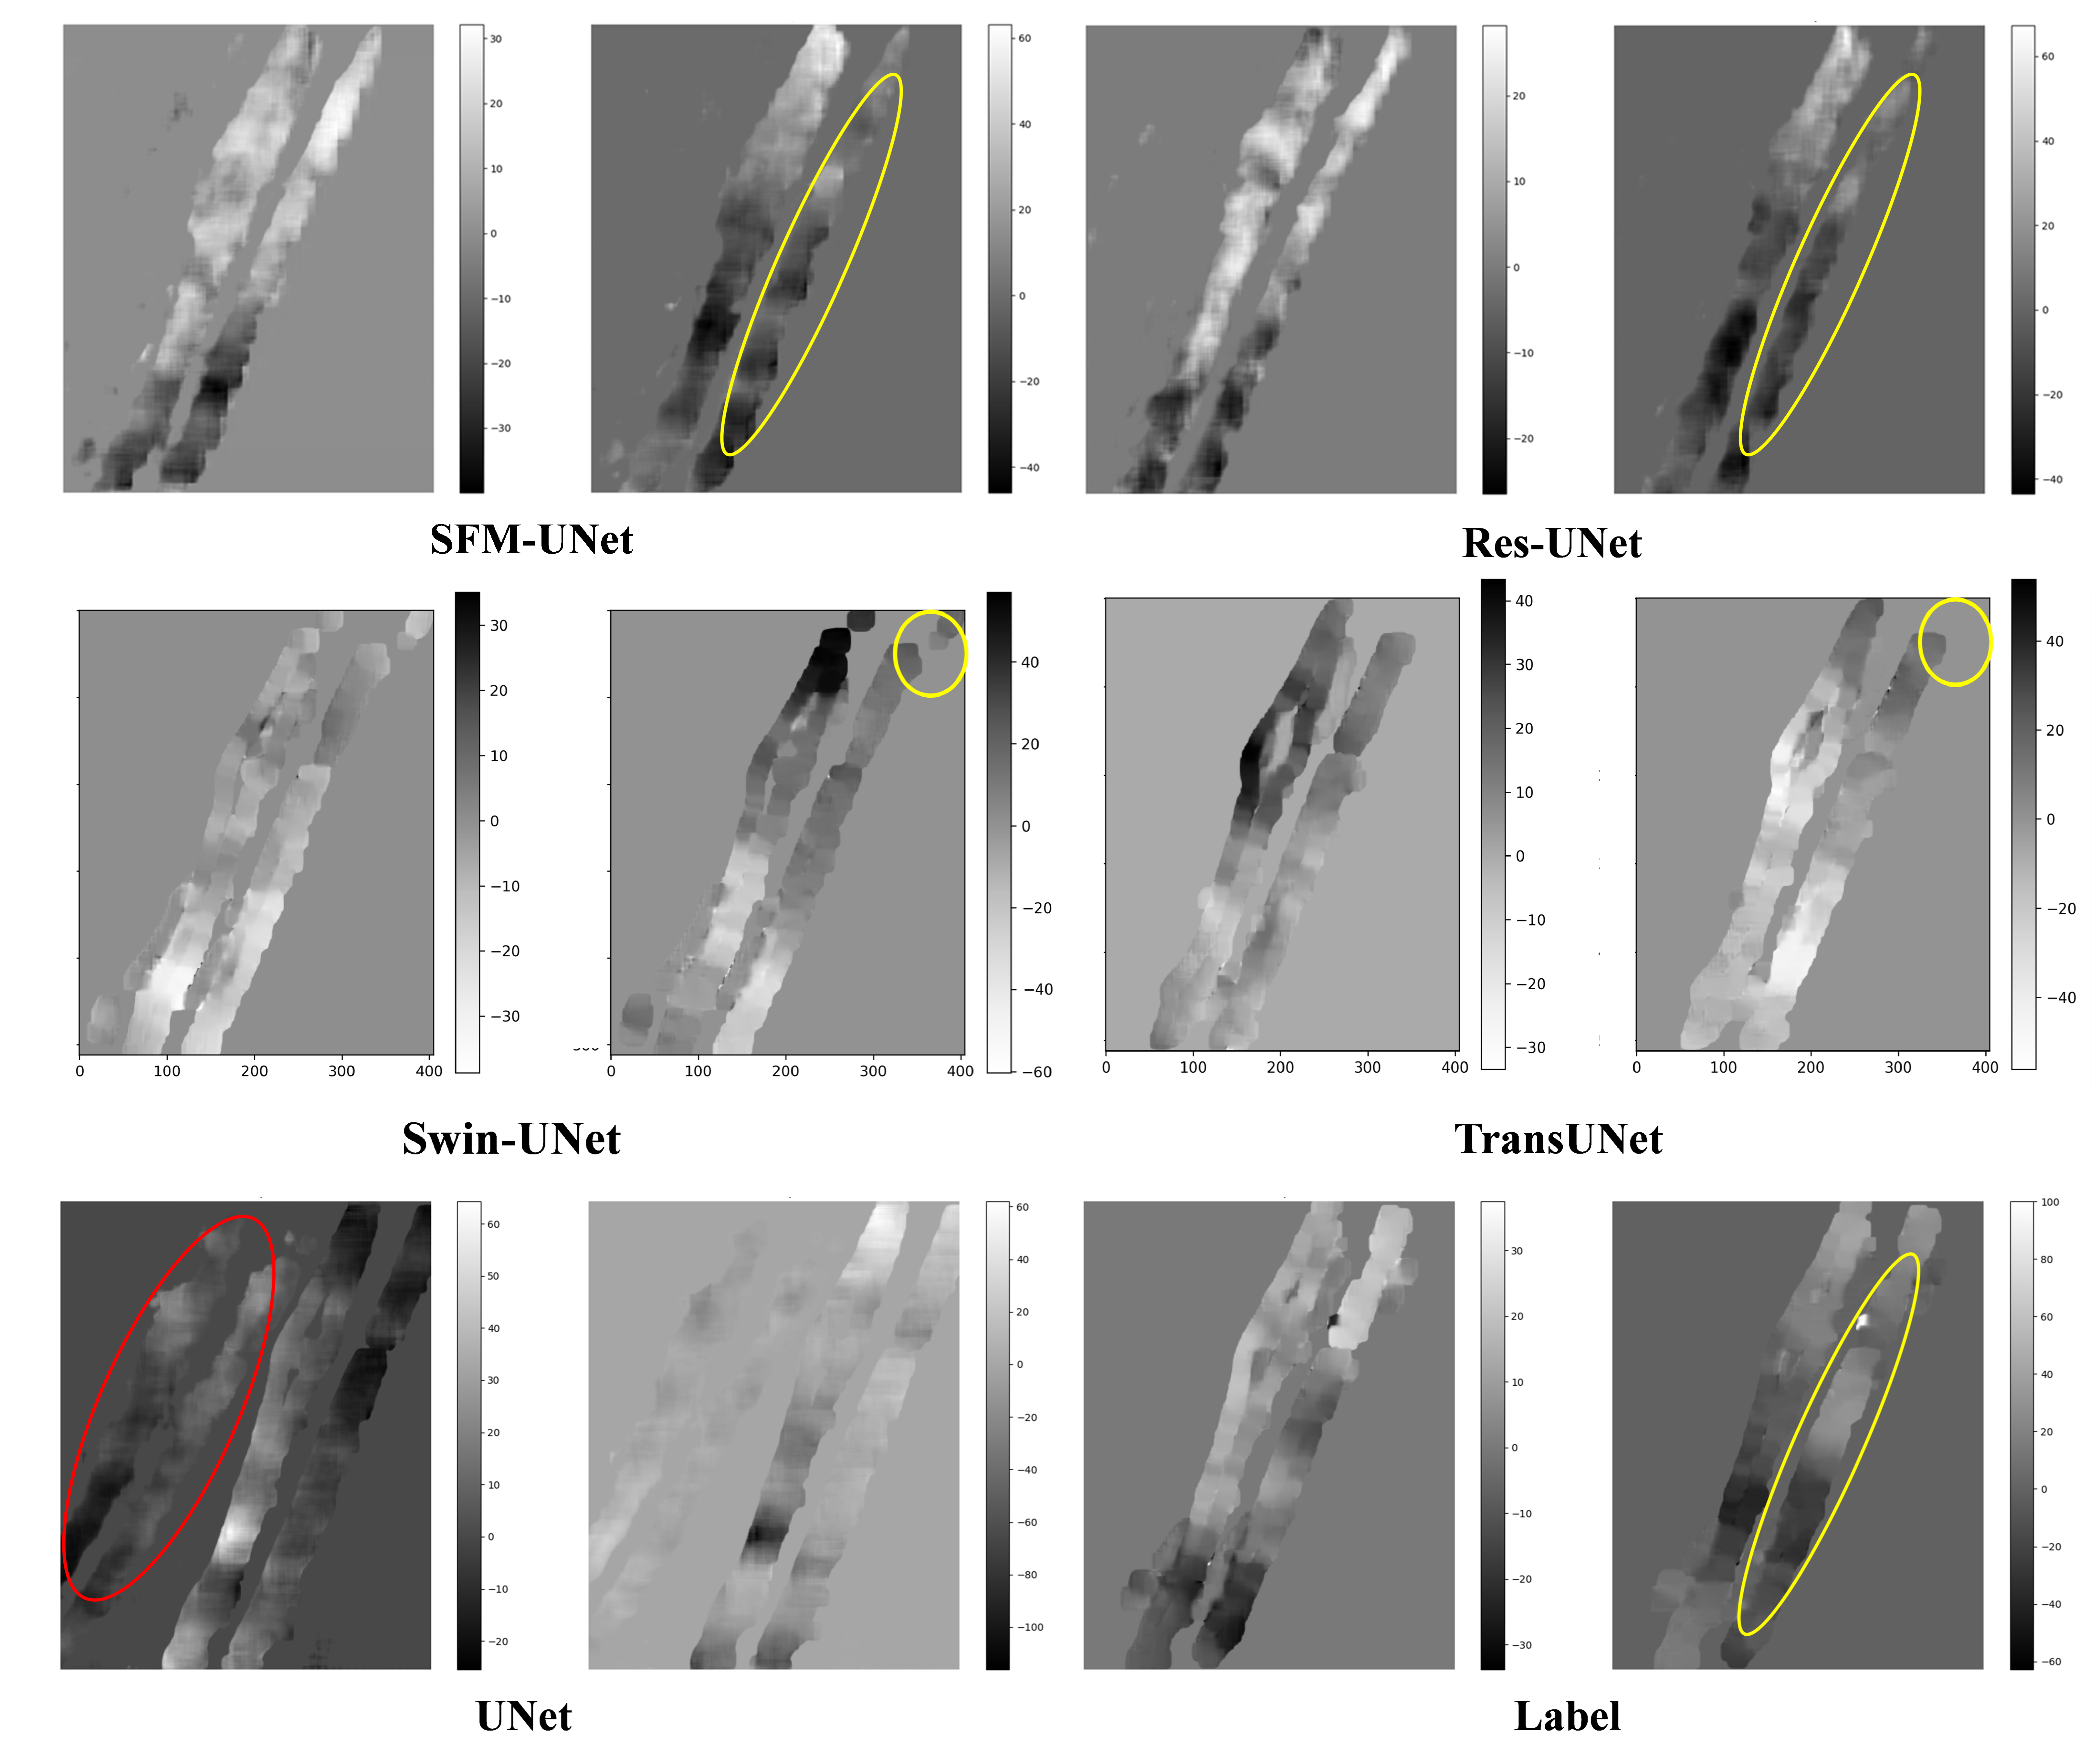
\includegraphics[width=0.9\linewidth]{Fig/fig3.png}}
\caption{Comparison of SFM-Unet and baseline models on posterior scleral OCT images.}
\label{fig:3}
\end{figure}

\subsection{Ablation experiments}
We conducted ablation experiments on the proposed SFM-Unet by systematically evaluating the impact of each individual component on the overall performance of the model, and the results are shown in Table~\ref{tab:comparison_settings}. In Settings I and III, the results are suboptimal due to the removal of the ECSFMB module, which results in the inability to utilize the spatial information. Furthermore, Setting II is less effective in comparison to SFM-Unet due to the failure to incorporate frequency information, which results in its inability to utilize global information and to recognize the crucial information embedded in the frequency domain.
\begin{table}[htbp]
\centering
\scriptsize
\caption{Comparison of different settings on the proposed SFM-Unet}
\begin{tabular}{lcccc}
\toprule
\textbf{Settings} & \textbf{FFF} & \textbf{ECSFMB} & \textbf{MAE$\downarrow$} & \textbf{MSE$\downarrow$} \\
\midrule
I & - & - & 0.12 & 6.038 \\
II & - & $\checkmark$ & 0.06 & 3.632 \\
III & $\checkmark$ & - & 0.09 & 4.019 \\
\midrule
SFM-Unet & $\checkmark$ & $\checkmark$ & 0.04 & 3.038 \\
\bottomrule
\end{tabular}
\label{tab:comparison_settings}
\end{table}

\section{Discussion}
The proposed SFM-Unet demonstrates significant advancements in posterior scleral OCT analysis by effectively addressing the dual challenges of spatial continuity preservation and computational efficiency in 3D medical image processing. Our experimental results on both the private EyePS2024 dataset and the publicly validated BraTS2020 benchmark underscore the model’s ability to balance segmentation accuracy with parameter efficiency, while its innovative architectural design offers new insights into multimodal feature fusion for medical imaging tasks.

With merely 5.51 million parameters, 80\% fewer than TransUNet (105.28M) and 49\% fewer than Swin-UNet (27.17M), SFM-Unet achieves competitive segmentation accuracy while drastically reducing memory consumption. This efficiency is attributed to the decoupled processing of spatial-frequency features and cross-slice dependency modeling, which circumvent redundant 3D convolution operations inherent in conventional volumetric networks. These characteristics render SFM-Unet particularly suitable for deployment in resource-constrained clinical environments where access to high-end GPUs remains limited, thereby bridging the gap between advanced computational methods and real-world medical infrastructure.  

Future work will explore combining complementary imaging modalities (e.g., OCT ocular angiography) to improve diagnostic accuracy. In addition, incorporating patient-specific biomechanical parameters into the model will enable predictive diagnosis of myopia progression.

\section{Conclusion}
Our proposed SFM-Unet offers a promising solution for the mechanical analysis of the posterior sclera of the eye by effectively addressing the loss of spatial information and the underutilization of information during 3D data slicing. The incorporation of frequency features and the Enhanced Cross-Slice Spatial-Frequency Memory Block (ECSFMB) module enables SFM-Unet to fully leverage both spatial and frequency information, thereby facilitating precise analysis on devices with constrained hardware resources. Our extensive experiments on the private dataset EyePS2024 and the public dataset BraTS2020 have demonstrated that our method is state-of-the-art. We will further explore combining complementary imaging modalities to improve diagnostic accuracy. %The substantial enhancements in the experimental outcomes serve to reinforce the efficacy and prospective value of SFM-Unet.



%\backmatter
\bmsection*{Author contributions}
Jiashu Xu: Conceptualization, Methodology, Software, Visualization, Validation, Writing – original draft. Fanglin Chen: Supervision, Writing – review \& editing, Project administration

\bmsection*{Conflict of interest}
The authors declare no potential conflict of interests.

\bibliography{references}







%\nocite{*}% Show all bib entries - both cited and uncited; comment this line to view only cited bib entries;


\end{document}
